\documentclass[a4paper]{article}
%\usepackage{inputenc}
\usepackage{csquotes}
\usepackage[margin=1.5cm]{geometry} % Change the margins
\usepackage[utf8]{inputenc} % - Defines what coding LaTeX uses. Use this one.
\usepackage[english]{babel}
\usepackage[T1]{fontenc}
\usepackage{graphicx} % - Package for including images in the document.
\usepackage{amsmath}
\usepackage{amssymb}
\usepackage{mathtools}
\usepackage{listings}
\usepackage{textgreek}
\usepackage{caption} % Correct spacing for captions
\usepackage{siunitx} % Package for handling numbers (ex \num{1e6}), units (ex \SI{15,3}{Nm}) and intervals (ex \SIrange{10}{20}{\celcius}) correctly
\sisetup{output-decimal-marker={,},range-phrase=--,range-units=single,exponent-product=\cdot} % If you write in English, remove output-marker...
\graphicspath{ {Images/} } % - Path to where the images are located on your computer. In this case I have a folder (look to the left) "Images" where the images are gathered.
\usepackage{hyperref} % - Package for including hyperlinks in the document.
\usepackage[style=apa,backend=biber]{biblatex} % APA-referenser
\usepackage{mhchem}
\DeclareLanguageMapping{swedish}{swedish-apa}  % APA-referenser
 % - Package for the bibliography ("referenser").
\addbibresource{references.bib} % - From where, i.e. which file, the references are taken. The bibliography file is called name.bib; see left column.

\title{TCP/IP Attacks}

\author{
Klas Mannberg \\
{klaman-8@student.ltu.se
} \\ \\

\includegraphics[width=0.2\textwidth]{ltu_swe.jpg}}
\date{24 September 2020}

\begin{document}

\maketitle


\tableofcontents


\section{Lab Tasks}
\subsection{Task 1: SYN Flooding Attack}
Spam start 3-way TCP handshakes on transport layer (TCL handshake on the app layer). Floods with requests asking for replies. \\
We create three virtual machines (hosts): Client/Attacker/Server. \\
After I retrieved the IP address of my server VM box, I launched a synflood attack using netwox 76 from the attacker VM. 
\ The result was many more half-open connections on the server. The connections before the attack are shown in image \ref{task1_before} and after in image \ref{task1_after}.

When the SYN flood was running from the attacker, the client could not telnet connect to the server anymore. See image \ref{task1_cantconnect}.
When I turned on SYN cookies on the server it no longer blocked the clients connection via telnet.\\
The cookies prevent the server from sending back the response SYN+ACK back until it receives a response ACK which an attacker never sends out with a normal SYN flood. This however opens a new attack to send many ACK's so the server gets overloaded anyway. To prevent this the server calculates the hash from the previous SYN+ACK and see if its a response from someone it has sent an SYN+ACK to, if its not it can just discard it and not waste resources.\\
\subsection{Task 2: TCP RST Attacks on telnet and ssh Connections}
Using the netwox 78 command with the filter parameter, we send out one RST packet for each packet from server host with the command. $sudo\ netwox\ 78\ --filter\ "src\ host\ 10.0.2.9"$ The result is the telnet (TCP) connection closing, as seen in image \ref{task2}.

The values were retrieved using wireshark on the attacker VMbox.
\subsection{Task 3: TCP RST Attacks on Video Streaming Applications}
Doing Task 2 but targeting the TCP connection of a video streaming service, \textit{Youtube}. The result is the video stops downloading and only the downloaded buffer remains. Eventually this leads to an error response from the video player.
\subsection{Task 4: TCP Session Hijacking}
I ran wireshark to find the appropriate parameters to make sure my packet is accepted. But also I made sure to be the next packet by assigning my packet the calculated next sequence number, given by wireshark. \
After I got the needed values for customizing our packet, I created the program shown in in image \ref{task4_code}.

In the image \ref{task4} you can see the server accepting my packet with the custom data!
\subsection{Task 5: Creating Reverse Shell using TCP Session Hijacking}
In this taks we repeat task 4 but with a command that launches a shell session for us! To accomplish this I use the same code as in Task 4 but change the data inside into a command that launches a shell using a port that I can connect to. After I retreived the necessary information from wireshark I got the server to run the reverse shell command via our spoofed packets! See image \ref{task5} for the attacker perspective. The client connection is frozen while we have access to SHELL.
\section{Images}
\begin{figure}[h]
    \caption{Task 1: Connections to server before SYN flood}
    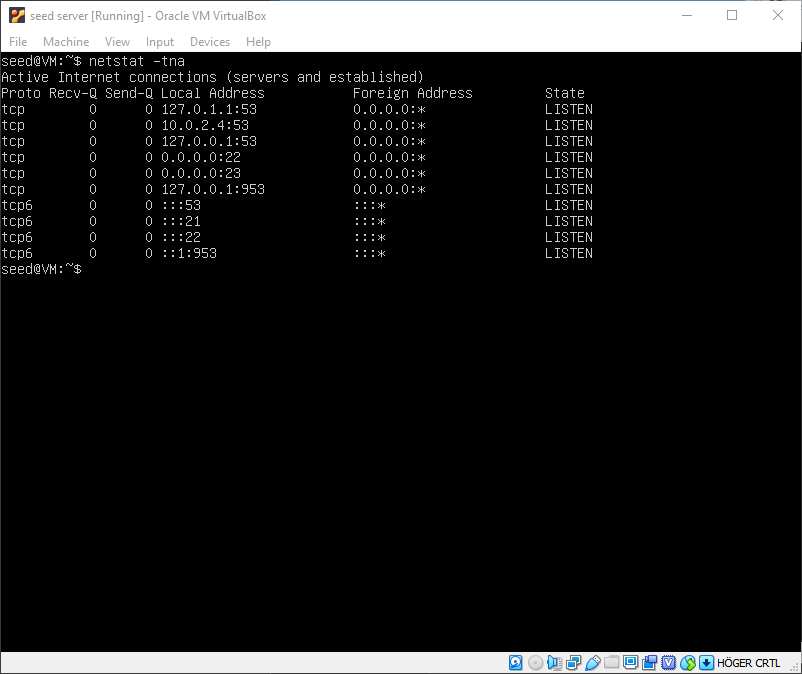
\includegraphics[width=\textwidth]{task1_before.png}
    \label{task1_before}
\end{figure}
\begin{figure}[h]
    \caption{Task 1: Connections to server after SYN flood}
    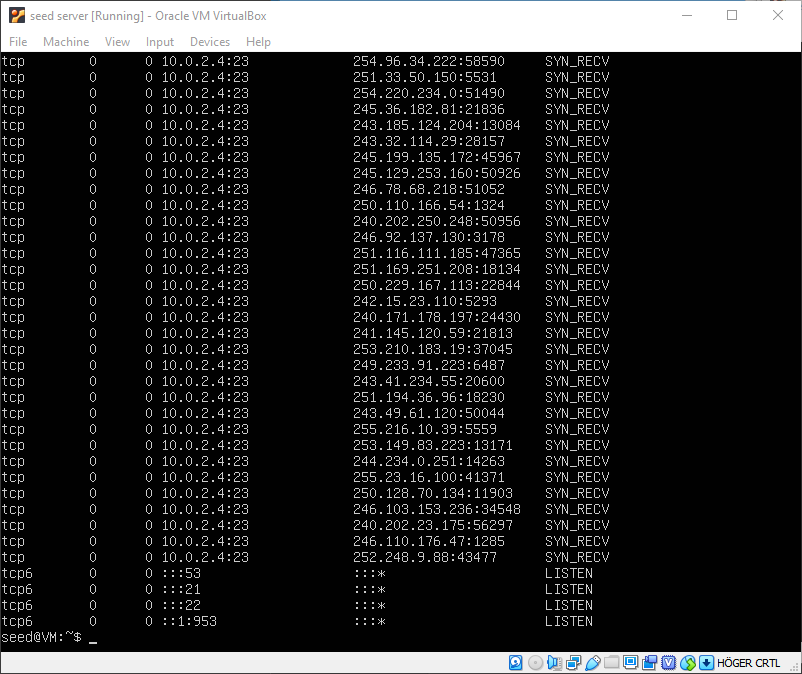
\includegraphics[width=\textwidth]{task1_after_nocookie.png}
    \label{task1_after}
\end{figure}
\begin{figure}[h]
    \caption{Task 1: Client tries to connect to server under SYN flood attack}
    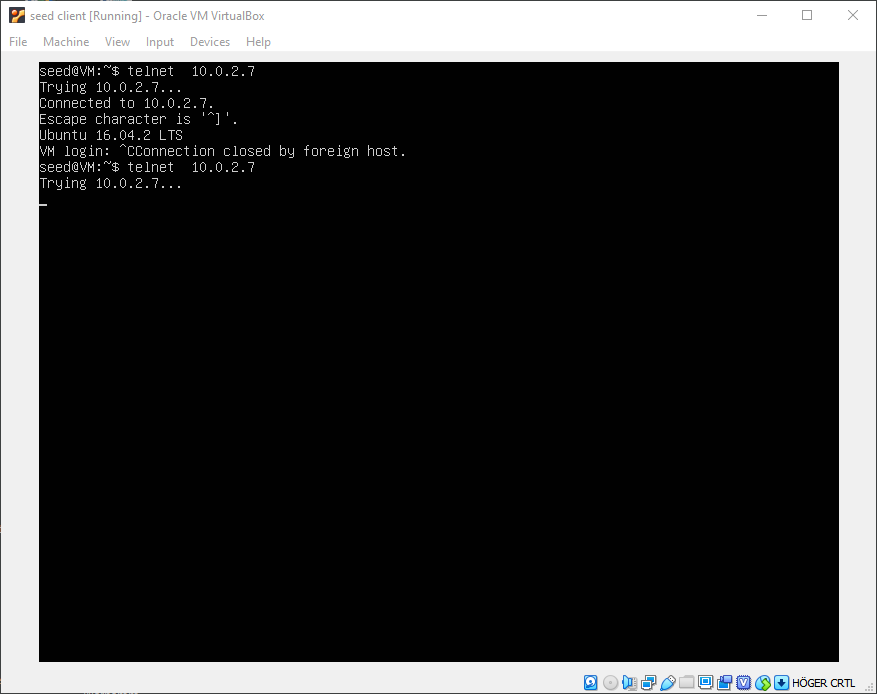
\includegraphics[width=\textwidth]{task1_cantconnect.png}
    \label{task1_cantconnect}
\end{figure}
\begin{figure}[h]
    \caption{Task 2: Disrupted telnet (TCP) connection!}
    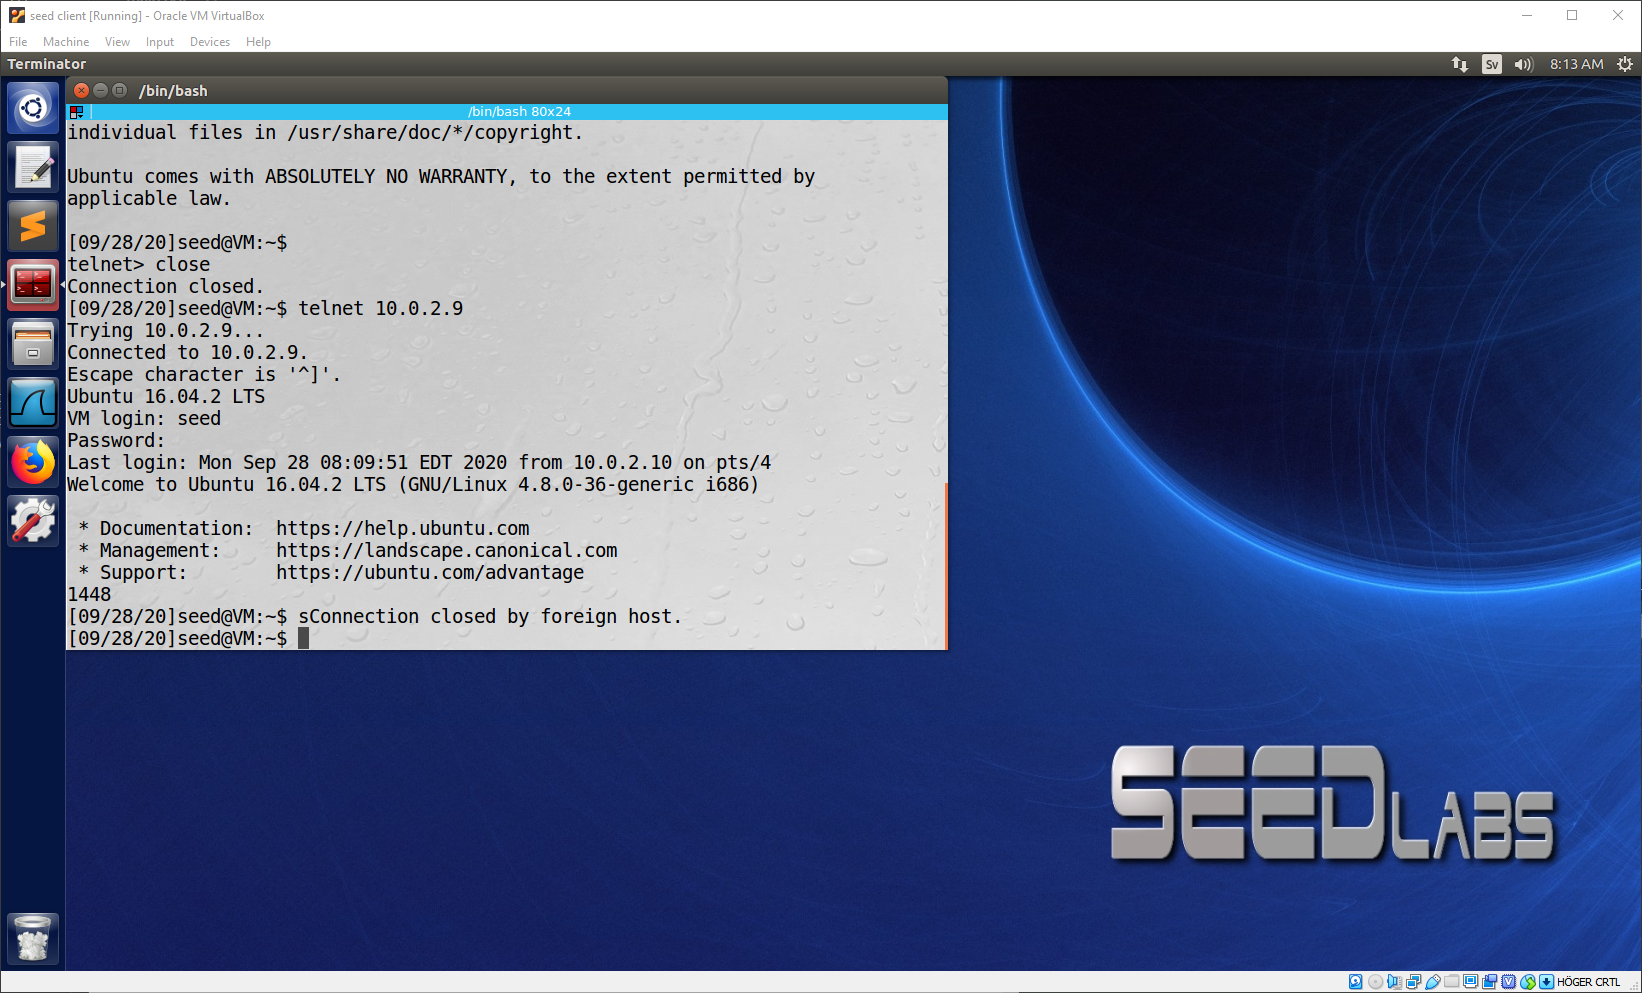
\includegraphics[width=\textwidth]{task2.png}
    \label{task2}
\end{figure}
\begin{figure}[h]
    \caption{Task 4: Source Code}
    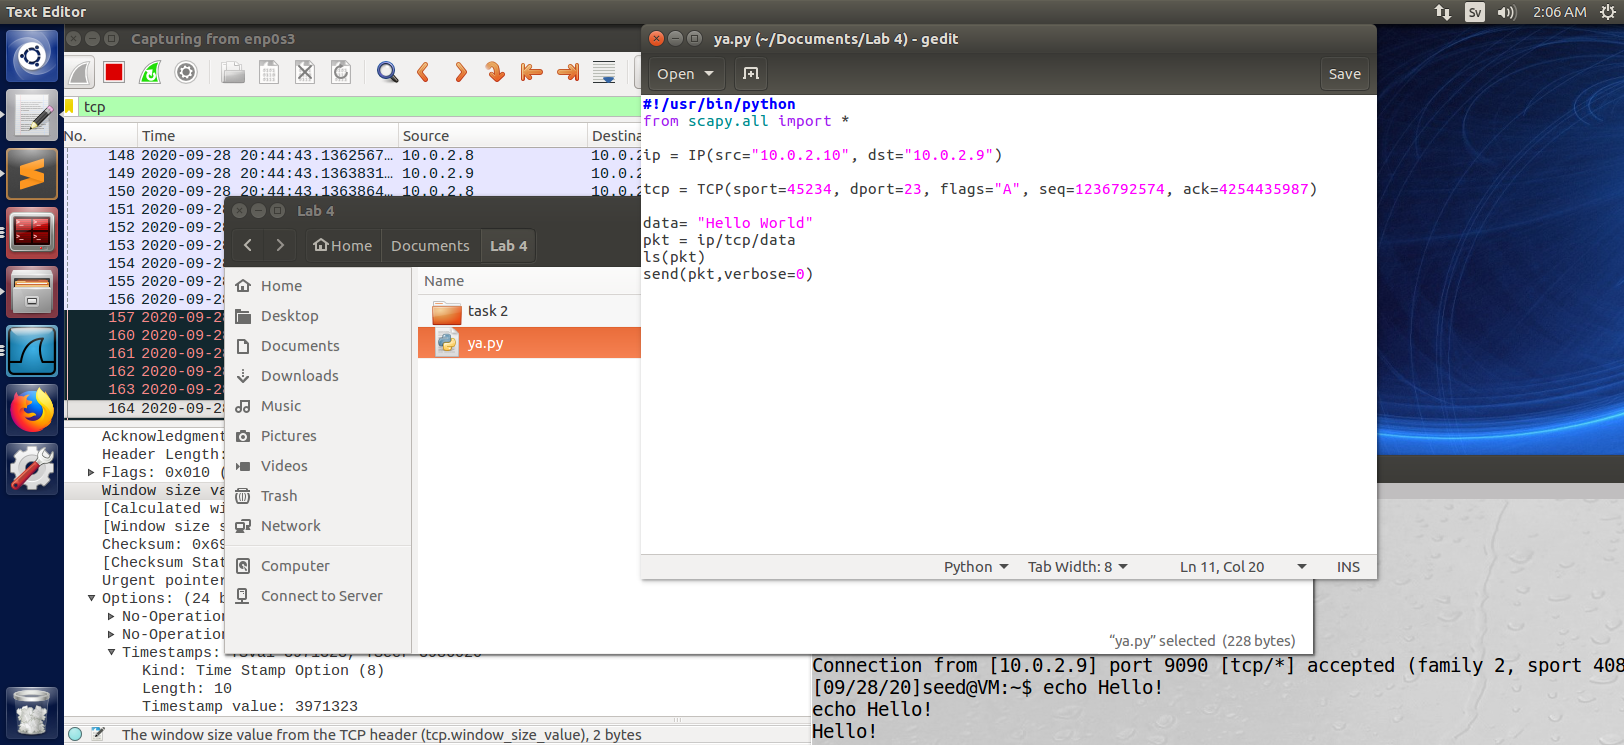
\includegraphics[width=\textwidth]{task4_code.png}
    \label{task4_code}
\end{figure}
\begin{figure}[h]
    \caption{Task 4: Sent data "Hello World" via TCP connection!}
    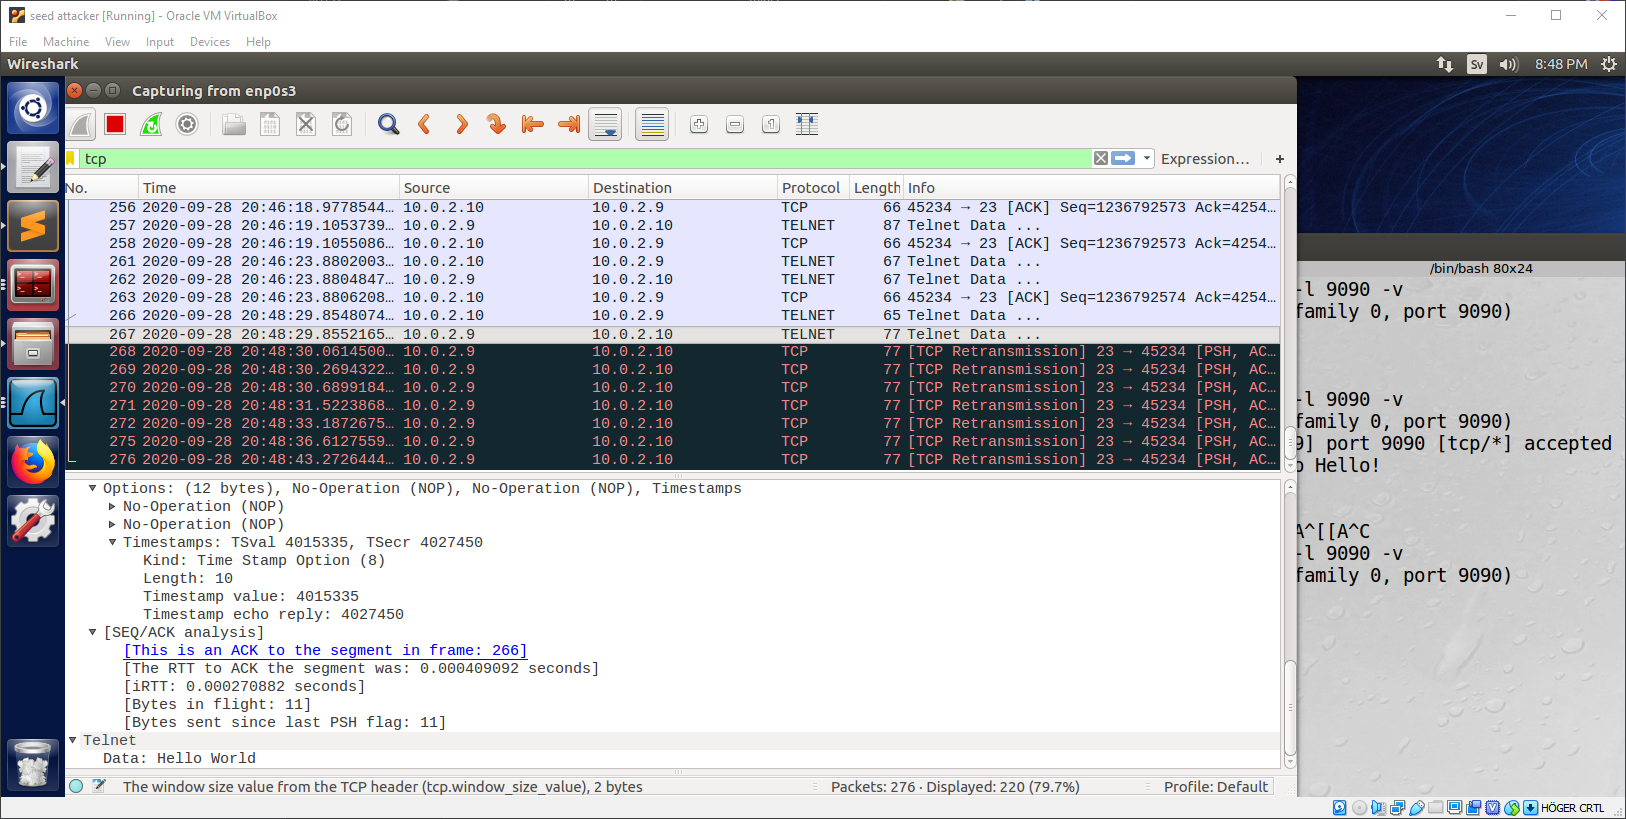
\includegraphics[width=\textwidth]{task4_2.png}
    \label{task4}
\end{figure}
\begin{figure}[h]
    \caption{Task 5: Got the server to run the reverse shell command}
    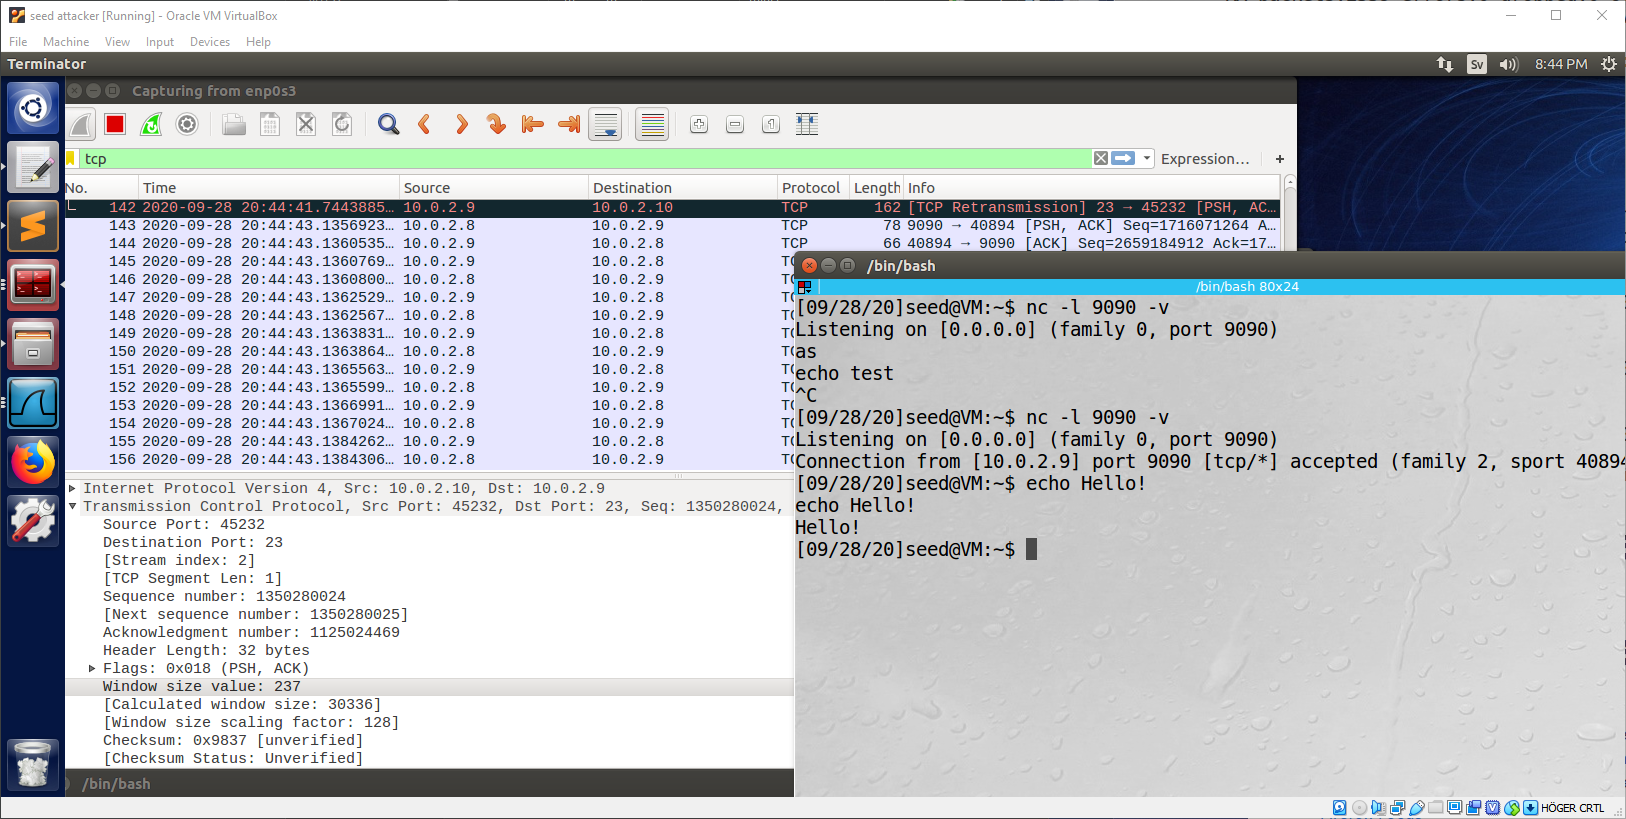
\includegraphics[width=\textwidth]{task5_2.png}
    \label{task5}
\end{figure}
\end{document}
